 \clearpage
 \setcounter{page}{1}
\section{Tensorrechnung und Kontinuumsmechanik \label{sec:tenkon}}


\subsection{Tensormultiplikation}

Schreiben Sie die folgenden Ausdrücke in Indexnotation und vereinfachen Sie soweit es geht.

\vspace{0.4cm}
\enab
\begin{minipage}[t]{0.5\textwidth}
 \item $\bI \dblc (\bA \otimes \bb)$
% \item $(\bA \smpc \bB)^T \dblc (\bc \otimes \bD)$
\item $(\bI \otimes \bI)^{T23} \dblc \bB $
% \item $ (\bA \otimes \bB)^{T23} \tplc (\bI \otimes \ba)$
\item $\bB \dblc (\bA\otimes \bA^T)\dblc \IL \dblc (\bB \otimes \bB^T) \dblc \bA$
\end{minipage}
%
\begin{minipage}[t]{0.42\textwidth}
\item $\bI \smpc (\bA \smpc \bB) $
\item $(\bI \otimes \bI ) \dblc \bB$
\item $\bA^T \dblc \IA  \dblc \bB$
% \item  $(\bA \smpc \bB)^T$
% \item $ (\bA \otimes \bB^T)$
% \item $\bA \smpc \bB^T $
% \item $(\bA \smpc \bB)^T$
\end{minipage}
\enae



\subsection{Differentialoperationen}

Schreiben Sie die folgenden Ausdrücke in Indexnotation und vereinfachen Sie soweit es geht.

\vspace{0.4cm}

\enab
\begin{minipage}[t]{0.5\textwidth}
\item $\displaystyle\frac{1}{2}(\grad{\bv+\grad^T\bv)}\dblc \bA$ (Ann.: $\bA=\bA^T$)
\item $\div{(\bv\smpc\bT)}$
\item $\displaystyle\pp{(\tr{\bA})}{\bA}$
\end{minipage}
%
\begin{minipage}[t]{0.42\textwidth}
\item $\displaystyle\pp{\bA}{\bA} \dblc \bB $
\item $\tr(\grad{(\bv\smpc\bT)})$
\item $\displaystyle\pp{(\bA \smpc \bB)}{\bA}$
% \item $\displaystyle\pp{(\bA \dblc \bB)}{\bA}$
\end{minipage}
\enae



\subsection{Elastizitätstensor und Voigt-Notation}

Für linear elastisches isotropes Material lässt sich der Elastizitätstensor $\IC$ wie folgt darstellen:
\eb \IC=\lambda\, \bI \otimes \bI + 2 \mu \, \II \label{eq:ic}\ee

\enab
\item Zeigen Sie, dass die Ausdrucksweisen
$ \Bsigma=\lambda \, (\tr{\Bvarepsilon})\,  \bI + 2 \mu \, \Bvarepsilon $ und 
$\quad \Bsigma= \IC \dblc \Bvarepsilon $
äquivalent sind.
Setzen Sie dazu \eqref{eq:ic} ein, schreiben die beiden Ausdrücke in Indexschreibweise und vereinfachen Sie soweit wie möglich.

\item Schreiben Sie das Materialgesetz $\Bsigma= \IC \dblc \Bvarepsilon$ zunächst in genereller Matrixnotation und dann in Voigt-Notation.
Unter welchen Annahmen ist dies möglich?
\par \textit{Hinweis}: $\Bvarepsilon$ lautet in Voigt-Notation $\Mvarepsilon^V=[\e_{11},\,\e_{22},\,\e_{33},\,2\e_{23},\,2\e_{13},\,2\e_{12}]^T$
\enae



\clearpage
\subsection{Analytische Lösung eines Randwertproblems}

Der dargestellte Körper $\B=l\times l\times t$ liegt reibungsfrei auf einer Ebene und ist im Koordinatenursprung (mittig in der $l$-$t$-Ebene) zusätzlich in Horizontalrichtung fixiert.
Auf ihn wirkt die Flächenlast $q$. 
Volumenkräfte durch die Erdbeschleunigung sind zu vernachlässigen.


\begin{center}
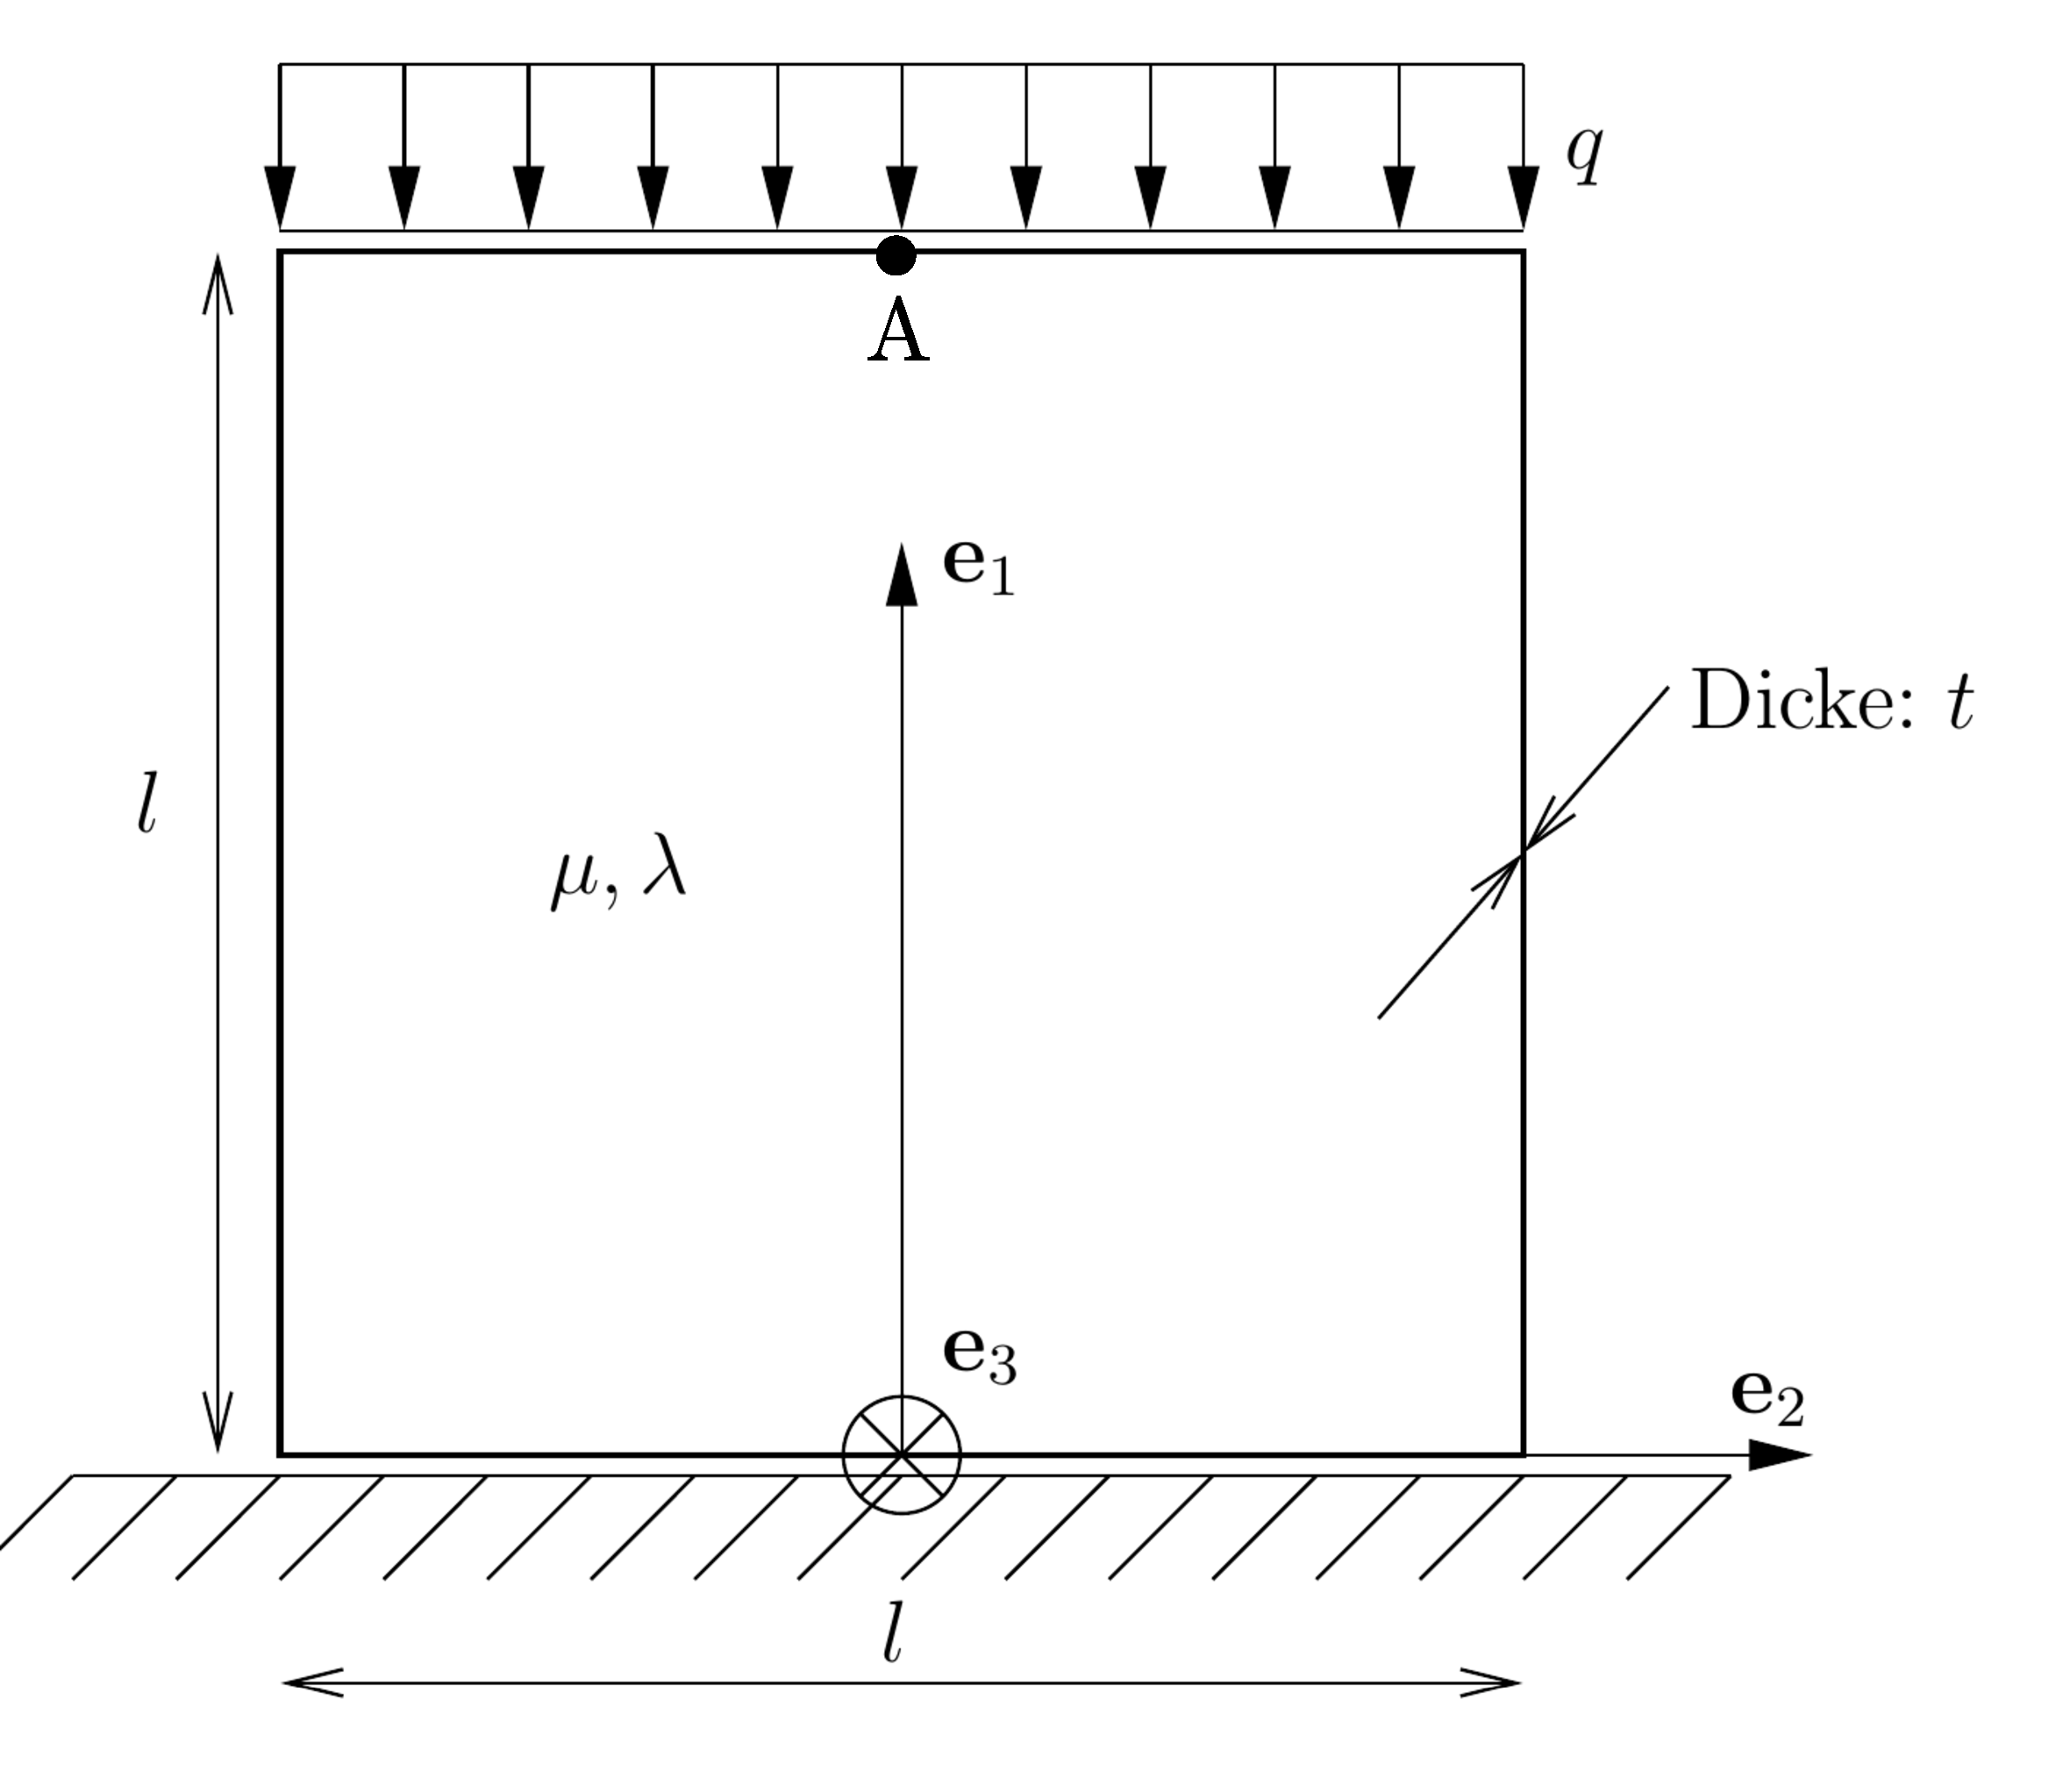
\includegraphics[width=0.6\textwidth]{fig/ue1_cube_surface_load_on_plane.pdf}
\end{center}


\enab
\item Erfüllt der Verschiebungszustand 
%$\mmu=[\alpha x_1 \,,\, \beta x_2 \,,\, \gamma x_3]^T$
$\bu= \alpha x_1 \be_1 + \beta x_2 \be_2 + \gamma x_3 \be_3$
die Impulsbilanz? 
Bestimmen Sie die Konstanten $\alpha, \beta, \gamma$ aus den Randbedingungen.
Nutzen sie dazu das Cauchy-Theorem $\Bsigma \smpc \bn=\bt$

\item Berechnen Sie die Verschiebung im Punkt A für den Parametersatz $\{E,\nu,q,t,l\}=\{210 \mrm{GPa},0.3,500 \mrm{MPa},100 \mrm{mm} ,100 \mrm{mm}\}$ 

\par \textit{Hinweis}: Die Beziehungen zwischen den Elastizitätsparametern lauten: 
\ebn \lambda=\frac{E \nu}{(1+\nu)(1-2 \nu)} \quad,\quad \mu=\frac{E}{2(1+\nu)} \een


\enae